\section{Humanoid Walking}
\label{sec::21_hw}
To get started with and to understand the presented concepts that generate dynamically balanced walking trajectories, we shall have a look at figure \ref{fig::2_cl} once more. The pattern generation therein (orange box), consists of four main building blocks: Forward kinematics, nonlinear model predictive control (NMPC), interpolation, and inverse kinematics. The relation between these four building blocks is shown in fig. \ref{fig::21_pg}.
\begin{figure}[h!]
	\centering
	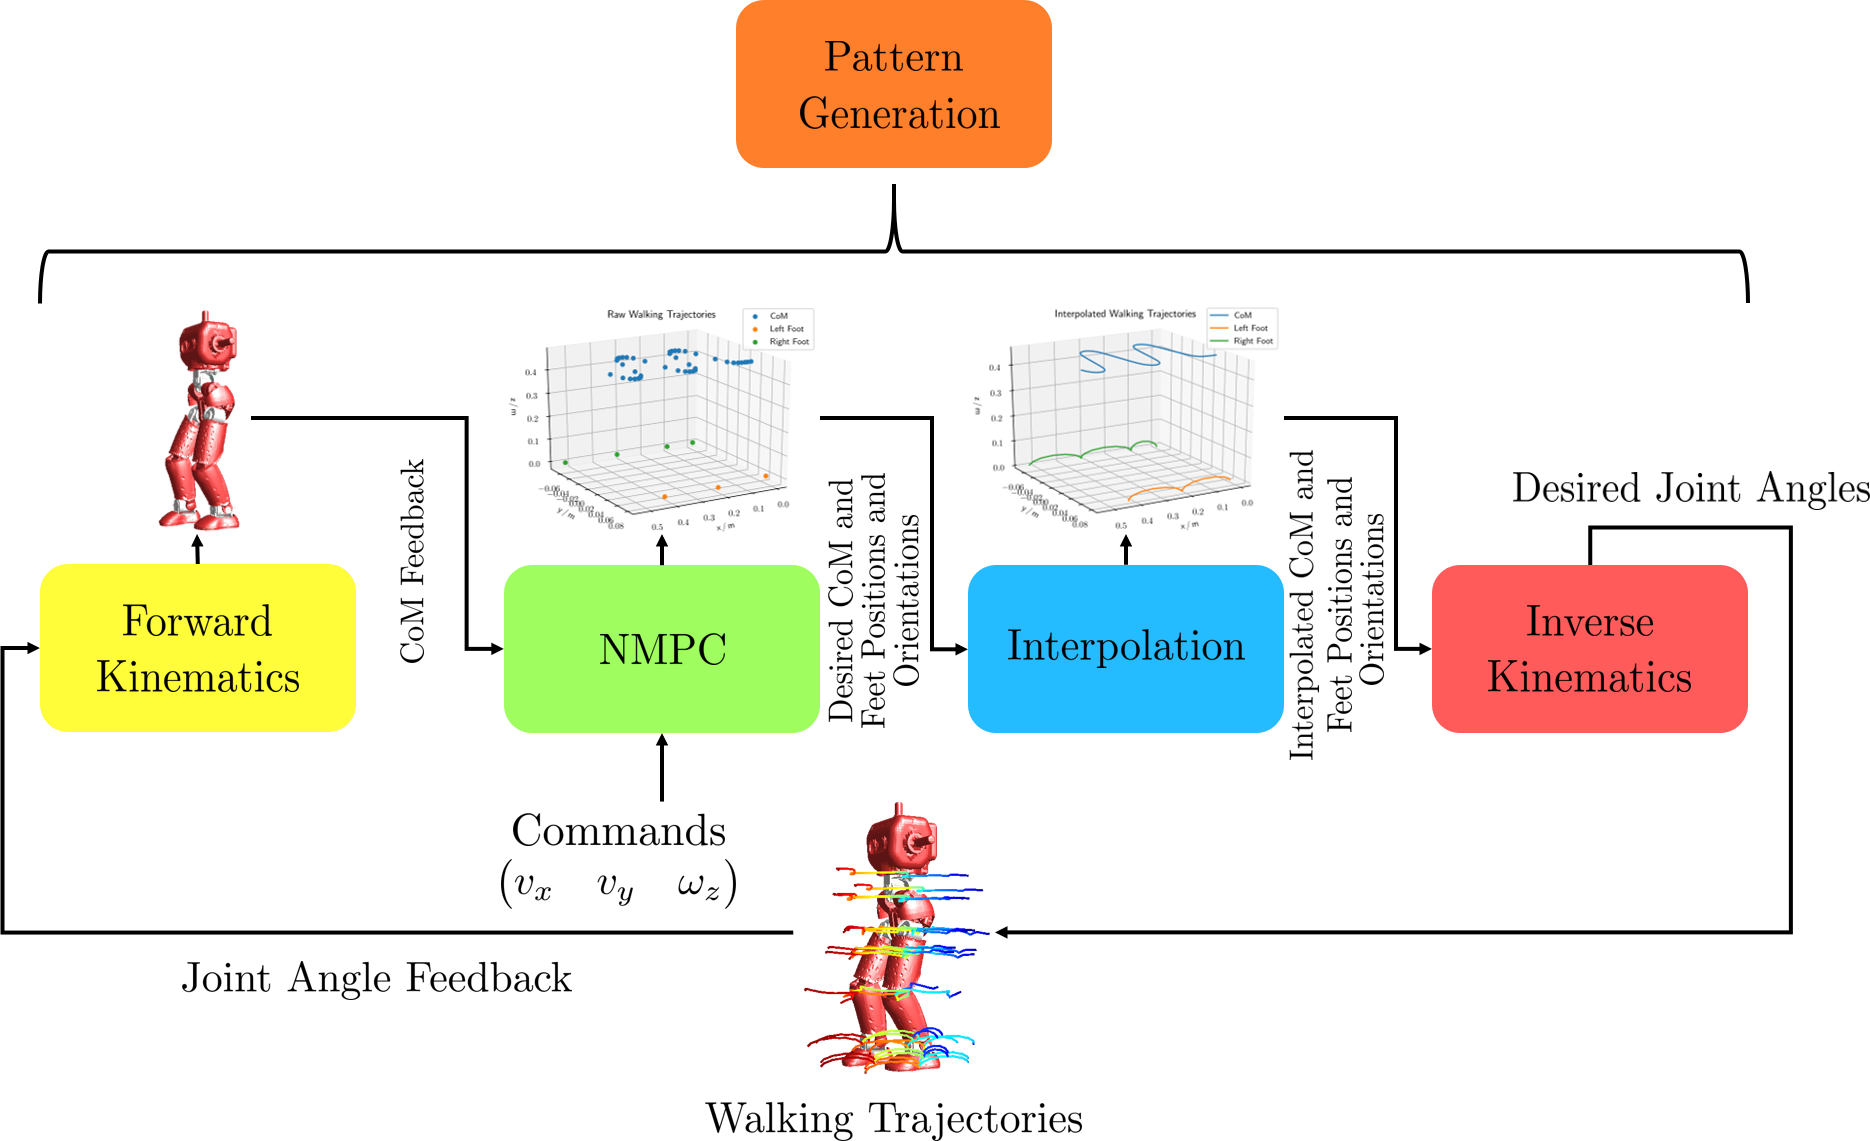
\includegraphics[scale=.5]{chapters/02_background/img/pattern_generation.png}
	\caption{Building blocks of the pattern generation. To understand the greater picture, a connection can be drawn to fig. \ref{fig::2_cl}, where the orange box represents the one shown in this figure.}
	\label{fig::21_pg}
\end{figure}
The natural entry point, to this otherwise closed control loop, is given by the commands that enter the nonlinear model predictive control. Commands are passed in the form of a desired velocity $\mathbf{v}_\text{ref}$ that the robot's center of mass (CoM) shall satisfy optimally according to a cost function that also takes dynamic balance and a smooth motion into account. The future desired positions and orientations for the CoM and the feet then result from the solution to a sequentially quadratic problem that tries to minimize this cost function. The balance criteria within this problem formulation is based upon the zero moment point (ZMP) around which the whole control framework is built. It is only by simplifying the robot's model that we can solve the optimal control problem in real time. Therefore, we assume the robot to be a linear inverted pendulum, for which we have a well defined analytical relation between the CoM and the ZMP. The minimization of the distance between the analytical expression of the ZMP and the foot placement results in the desired dynamic balance. As shown in fig. \ref{fig::21_pg}, the desired CoM and the feet positions and orientation, as they are obtained from the NMPC, are sparsely distributed in space. Moreover, there is neither information about how the feet shall move along the z-axis, nor along the x-, and y-axis, but only where they should be placed in the x-y-plane. Therefore, as the subsequent step to the NMPC, we need to add an interpolation. The interpolation interpolates the trajectories of the CoM to obtain a finer sampling time. Additionally, the movement of the feet in the x-, y-, and z-direction, as well as their orientation, is computed by polynomials that we require to satisfy the initial and end conditions of the foot placement. Put together, the nonlinear model predictive control and the interpolation between the resulting subsequent solutions for the positions and orientation of both, the CoM and the feet, describe dynamically balanced trajectories, given that the humanoid robot of interest resembles the physics of an inverted pendulum. Now to bridge the gap between dynamically balanced trajectories in Cartesian space, and a humanoid robot that actually satisfies them with its CoM and its feet, the inverse kinematics problem needs to be addressed. The inverse kinematics, which follow immediately after the interpolation step, take the positions and orientations of the CoM and the feet as constraints and find a composite of joint angles that fulfill them. The continuity of subsequent solutions is therein assured by initializing the inverse kinematics with the previous solution. Resulting joint angles, once passed to the humanoid, then result in walking trajectories, as indicated in fig. \ref{fig::21_pg} by the colored lines at the joints of the robot. Due to the inherent mismatch of the robot's physics from that of an inverted pendulum, as well as other effect like friction, there is a chance that the desired joint angles differ from the actually achieved ones. To compensate for the discrepancy, the last building block of the pattern generation is the feedback of the measured CoM to the NMPC. The CoM is computed by reading out the achieved joint angles, so that the forward kinematics can be utilized to determine the positions and orientations of the humanoid's links in space, and therefore the CoM.
\\\\
As already highlighted in the previous paragraph, special attention has to be given to the zero moment point, since it defines the central concept of the presented pattern generation. We therefore will explain its theoretical foundations, as well as its analytical relationship to the CoM for simplified physical models, and ways to measure it with force torque sensors in the section that lies ahead - Zero Moment Point.





 